% !TEX useTabsWithFiles
% !TEX tabbedFile{./content/content-ulgr/Beitrag-ulgr.tex}(ulgr)
% !TEX tabbedFile{./content/content-abcd/Beitrag-ulgr.tex}(abcd)
% !TEX TS-program = pdflatexmk
%% ---------------------------------------------------
%% -- Stand: 2023/02/07
%% -- Datei für die Erstellung des Rom-Buchs
%% -- Wir nutzen KOMA-Script  
%% ---------------------------------------------------
\documentclass[%
	,ngerman				
	,bibliography 	= leveldown % nicht Chapter
%	,draft
%	,parskip = half+			
	]{scrbook}

%% -- KOMA Otions
%% -- 
\KOMAoptions{%
	,paper 		= a4
	,pagesize
	,BCOR		= 15mm		% siehe KOMA-Script 2.6, S. 39
	,twoside		= true		% siehe KOMA-Script 2.6, S. 47
	,fontsize	= 12pt		% Standard ist 11pt
% 	,DIV		= calc		% siehe KOMA-Script 2.6, S. 42
	,headings 	= small		% siehe KOMA-Script 3.16, S. 113
	}

%% -- Die Pakete für RomSeminar
%% -- Stand: 2023/02/02
%% -- Literatur: H. Voss, Einführung in LaTeX (7. Auflage) 2022 
%% -- Muss mal sehen, wie ich dieses besser machen kann
%% --




%% -- Aufzählungen
%% -- 
\usepackage[%
	,inline			% für Aufzählungen im Text = Sternvariante
	,shortlabels	% damit \begin{enumerate}[(i)] funktioniert
	]{enumitem}
	
%% -- tikz
\usepackage{tikz}
\usetikzlibrary{positioning,arrows}

%% -- Pakete mit Referenz
%% -- 
\usepackage[newcommands,footnotes,raggedrightboxes]{ragged2e}
	
\usepackage{% Voss, LaTeX - 6.3 - Seite 227ff					
	,array 			   	
	,booktabs
	,tabularx
	,wrapfig
	,longtable}
	
\RequirePackage{% Voss, LaTeX - 8.6 - Seite 340ff					
	,caption 			   	
	,floatrow
	,subcaption}

\RequirePackage{% 						
	,multicol	% Voss, LaTeX - 5.15.1 - Seite 215	
	,parallel	% Voss, LaTeX - 5.15.2 - Seite 216
	}
	 	   	
\RequirePackage{%
	,graphicx	% Voss, LaTeX - 5.10.2 - Seite 174
	,wrapfig	% Voss, LaTeX - 5.10.3 - Seite 177
	,cutwin		% Voss, LaTeX - 5.10.3 - Seite 178
	}

%% -- Wenn schon, dann muss man es auch definieren
%% -- 
\usepackage{nicefrac}

%% -- Zum Testen
%% -- 
\usepackage{blindtext,lipsum}

%% -- Für Rahmen
%% -- 
\usepackage{mdframed}
%% -- infobox
\newmdenv{infobox} %% \begin{infobox} .. \end{infobox}





\usepackage[
	,Rom2Buch
%	,Rom2Online
	]{./preamble/Rom-Buch}

%% -- Literaturverzecinis seprat bei jedem Beitrag
%% -- \begin{refsection} .. \end{refsection}
%% -- Es können die jewiligen bib-Dateinen verwendet werden
%% -- Bitte Pfad richtig setzen
%% --
%\addbibresource{./bib/Rom-Biblio.bib}
\addbibresource{./content/content-ulgr/bib-ulgr/Biblio-ulgr.bib}	
\addbibresource{./content/content-abcd/bib-abc/Biblio-ulgr.bib}	
%%
\ExecuteBibliographyOptions{%
	,backref		= false 		% true = was habe ich genutzt
 	,url		= true		% true: URL werden angezeigt
 	,doi		= false		% DOI werden im Titel hinterlegt 
	,eprint		= false		% true  - ” -
	}
	
%% -- Zusätzliche Definitionen; müssen eventuell
%% -- in eine gemeinsame Datei wegen doppelter Befehle
%% --
%% -----------------------------------------------------
%% -- Für die eigenen Definitionen
%% -- Stand: 2023/02/02
%% -- Wissen, was man macht ist notwendig
%% ----------------------------------------------------- 

%% -- Für was dokumentierens
%% -- 
%% -----------------------------------------------------
%% -- Für die eigenen Definitionen
%% -- Stand: 2023/02/02
%% -- Wissen, was man macht ist notwendig
%% ----------------------------------------------------- 

%% -- Für was dokumentierens
%% -- 

%% -- Links farbig etc.
%% --
\ifthenelse{\boolean{Rom2Buch}}
	{\hypersetup{hidelinks=true}} % für Buch keine Links
	{\hypersetup{% else für online
		,colorlinks	= true                                                          
		,urlcolor	= blue  %                                                              
		,citecolor	= blue  %                                                          
		,linkcolor	= blue	}}	 	

%% -- Einstellungen Dictum; siehe KOMA Seite 138-140
%% --
\renewcommand{\dictumwidth}{0.45\textwidth}

%% -- Wir starten nun
%% --
\begin{document}

%% -- Frontmatter
\frontmatter
\ifthenelse{\boolean{Rom2Buch}}
	{% !TEX root = ../Rom-Buch.tex
% ---------------------
% Titelseite Rom-Titel-Buch.tex
% Stand	: 2023/02/05
% ---------------------
\begin{titlepage}
%
\newcommand{\HRule}{\rule{\linewidth}{.25mm}}
\vspace*{\stretch{1}}
\HRule
\vspace*{10pt}
%%
\begin{center}
	{\scshape {\Huge Zufall} \\[0.5em]
	{\Large Annäherungen aus Mathematik und Informatik} \\[5mm]
	{\large Romseminar 2024} \\ }
	\vspace*{15pt}
	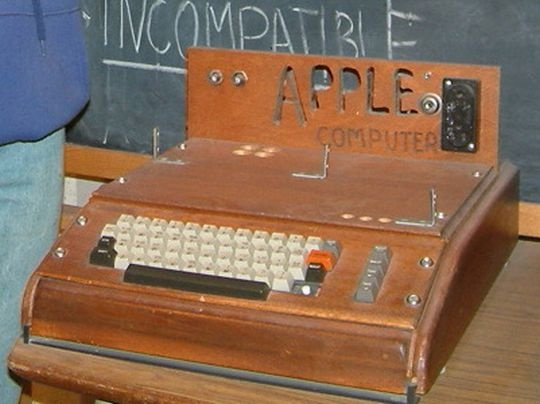
\includegraphics[width=14cm, height=12cm, keepaspectratio=true]{./content/Gruppenbild}
	\vspace*{10pt}	  
\end{center}
%
\HRule
\vspace*{\stretch{2}}
\begin{center}
	  {Version: \today }
\end{center}
\end{titlepage}
%% } 		% Titelseite für Buch
	{% !TEX root = ../Rom-Buch.tex
% ---------------------
% Titelseite Rom-Titel-Online.tex
% Stand	: 2023/02/05
% ---------------------
\begin{titlepage}
%%
\begin{center}
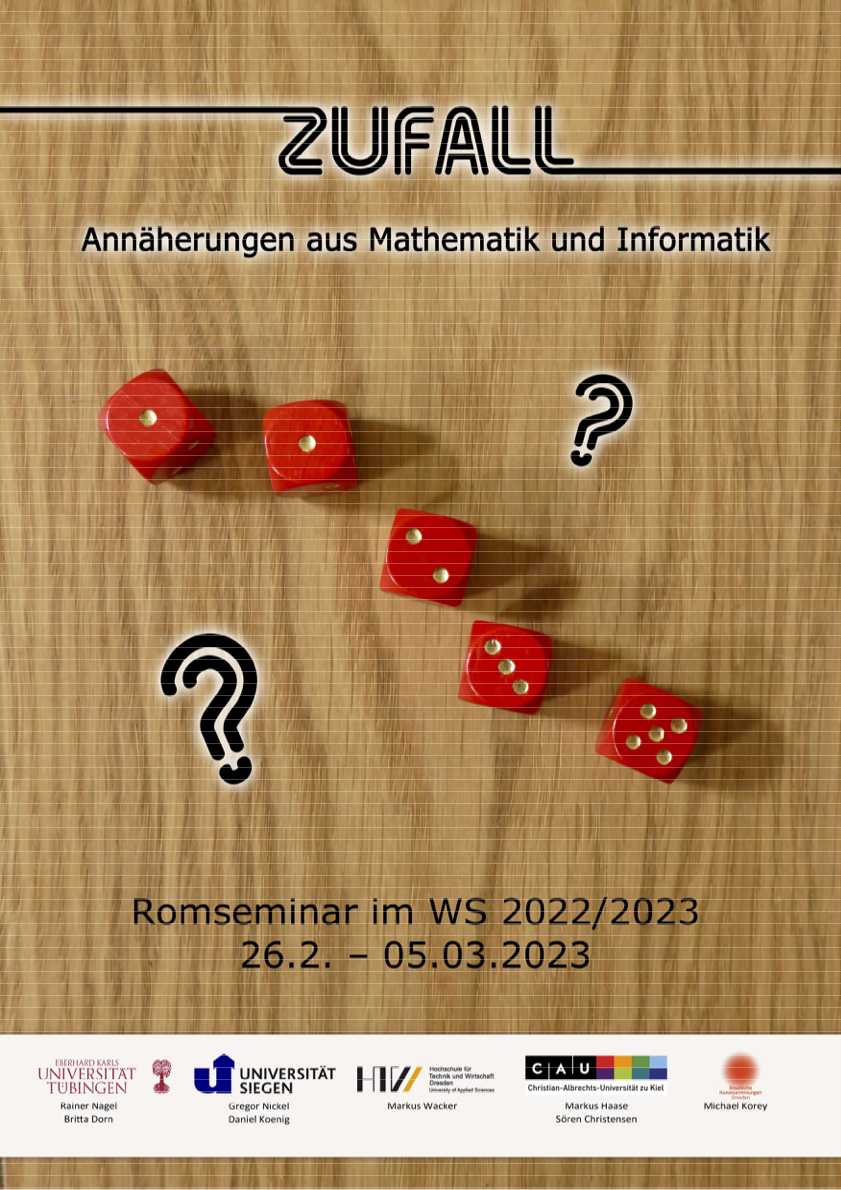
\includegraphics[width=14cm, height=28cm, keepaspectratio=true]{./content/Poster_Zufall.png}
\end{center}
\pagebreak
\vspace{2cm}
%% --
\thispagestyle{empty}
\newcommand{\HRule}{\rule{\linewidth}{.25mm}}
	\vspace*{\stretch{1}}
	\HRule
	\vspace*{10pt}
	\begin{center}
	{\scshape {\Huge Zufall} \\[.5em ]
	  {\Large Annäherungen aus Mathematik und Informatik} \\[5mm]
				{\large Romseminar 2023} \\ }
%	  	\enquote} \\[5mm]
%	  {\LARGE } \\[7.5mm]
	\vspace*{15pt}
	\includegraphics[width=14cm, height=12cm, keepaspectratio=true]{./content/gruppenbild}
	\vspace*{10pt}	  
	\end{center}
	%\end{flushright}
	\HRule
	\vspace*{\stretch{2}}
	\begin{center}
	  {Version: \today }
	\end{center}
\end{titlepage}
}	% Titelseite für online
%	% !TEX root = ../Rom-Buch.tex
% ---------------------
% Titelseite Rom-Titelseite.tex
% Stand	: 2023/02/02
% ---------------------
\begin{titlepage}
	\newcommand{\HRule}{\rule{\linewidth}{.25mm}}
	\vspace*{\stretch{1}}
	\HRule
	\vspace*{10pt}
	%\begin{flushright}
	\begin{center}
	  {\scshape {\Huge Zufall} \\
	  {\Large Annäherungen aus Mathematik und Informatik} \\[5mm]
				{\large Romseminar 2023} \\ }
%	  	\enquote} \\[5mm]
%	  {\LARGE } \\[7.5mm]
	\vspace*{15pt}
	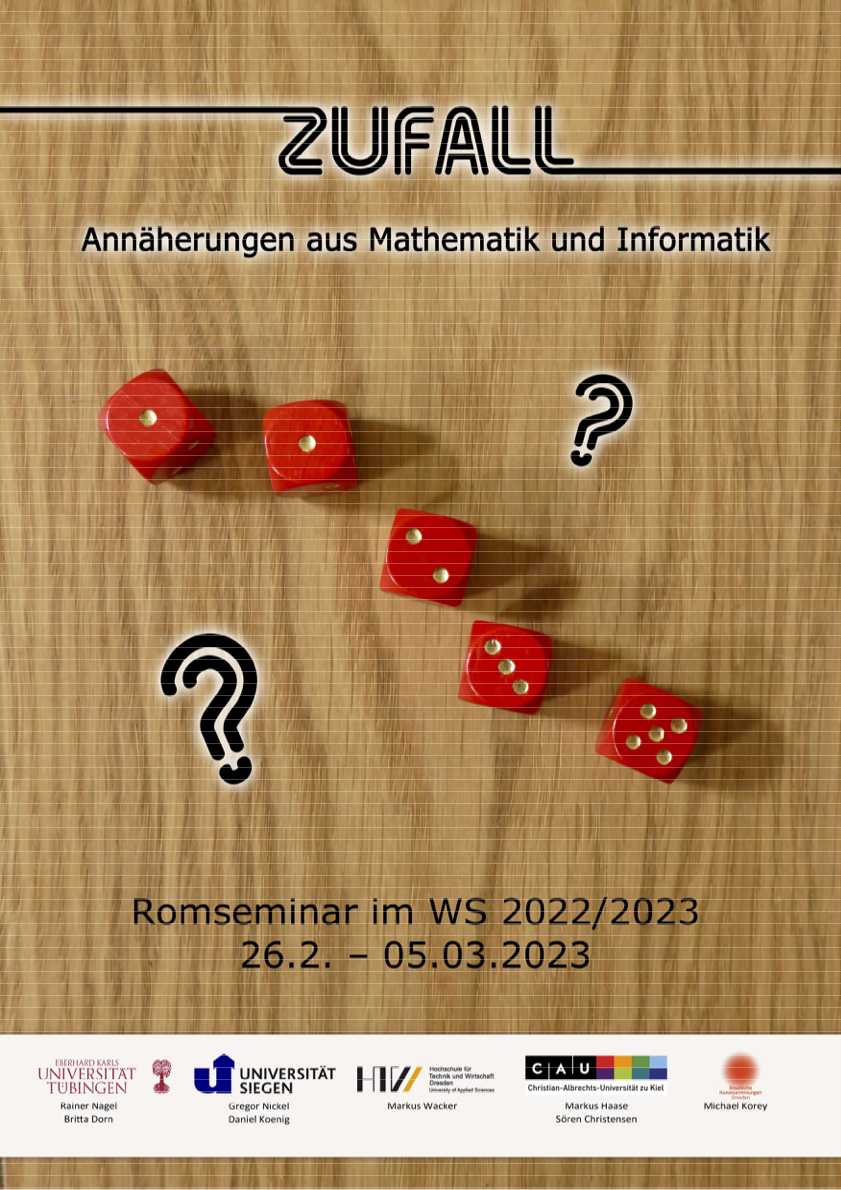
\includegraphics[width=14cm, height=12cm, keepaspectratio=true]{./content/Poster_Zufall}
	\vspace*{10pt}	  
	\end{center}
	%\end{flushright}
	\HRule
	\vspace*{\stretch{2}}
	\begin{center}
	  {Version: \today }
	\end{center}
\end{titlepage}

\tableofcontents
% !TEX root = ../Rom-Buch.tex
%% --
%% -- Rom-Vorwort.tex
%% --
\chapter*{Ein Vorwort}
\lipsum[1-2]
% !TEX root = ../Rom-Buch.tex
%% --
%% -- Rom-Agenda.tex
%% -- ulgr: Besser mit lontable dieses machen
%% --
\chapter*{Die Agenda}
%% mit longtable setzen
Hier folgt die Agenda

\begin{description}
\item {\textbf{Sonntag, xx. März 2023}}
\begin{itemize}
\item[~] {Ankunft in Rom, Bezug der Unterkunft, Kennenlernen beim Pizzaessen: 
   Pizzeria ``Wanted'' an der Ecke Via Leonina Via dei Serpenti} (ca. 19 Uhr)
\end{itemize}
\smallskip

\end{description}

%\item {\textbf{Montag, 26. September 2022 -- Accademia dei Lincei}}
%\begin{itemize}
%\item[ 9$^{30}$] { Begr\"u{\ss}ung, Vorstellungsrunde}
%\item[10$^{30}$] {\textbf{Anastasia Boushmelev \& Lukas Strauch:}} {\emph{Die Große Vereinheitlichung.}}
%\item[12$^{00}$] {\textbf{Nina Henn:}} {\emph{Zur unverständlichen Effektivität der Mathematik.}}
%\item[13$^{00}$] \hfill {\textsc{Mittagspause}} \hfill ~
%\item[14$^{00}$] {\textbf{Aaron Kettner:}} {\emph{Die Jagd auf Schrödingers Katze: Lieber tot als lebendig?}}
%\item[15$^{00}$] {\textbf{Alice Maurer:}} {\emph{Replizierbarkeit -- das Problem aller empirischen Wissenschaften.}}
%\item[16$^{00}$] {\textbf{ Cornelia Vogel \& Michael Zimmermann:}} {\emph{Es werde Licht – Quantengravitation 
%  und andere philosophische Ansichten über die Entstehung der Welt.}}
%\item[18$^{30}$] \hfill {Cena (Pizzeria Da Baffetto, Via del Governo Vecchio 114, Roma)}  \hfill ~
%%   \hfill  {\footnotesize Treffpunkt: Piazza Navona am mittleren Brunnen}\hfill ~
%\end{itemize}
%\smallskip
%
%
%%\newpage
%
%
%\item {\textbf{Dienstag, 27. September 2022 -- Accademia dei Lincei / Villa del Priorato di Malta}}
%\begin{itemize}
%\item[9$^{15}$] {\textbf{Hannes Wagener:}} {\emph{Ökonomie jenseits von Mark und Plan?}}
%\item[10$^{15}$] {\textbf{Maximilian Weinberg:}} {\emph{Die `überforderte Gesellschaft'.}}
%\item[11$^{15}$] {\textbf{Tobias Bungart, Dennis Loch \& Jannik Marcel Nöll:}}  {\emph{Verschwörungstheorien.}}
%\item[12$^{45}$] \hfill {\textsc{Mittagspause}}\hfill ~
%%\newpage
%
%\item[15$^{00}$] {\textbf{Ivo Graziani (Chief of Cabinet of the Grand Hospitaller):}}
%         {\emph{Der Malteserorden und seine harten Probleme.}}
%\item[16$^{30}$] {Besichtigung der Magistralvilla und der Prioratskirche (Piranesi).}
%\end{itemize}
%\smallskip
%
%\newpage
%
%\item {\textbf{ Mittwoch, 28. September 2022 -- Bibliotheca Hertziana (MPI für Kunstgeschichte)}}
%\begin{itemize}
%\item[9$^{00}$] {\textbf{Dr. Sietske Fransen:}} {\emph{Von der Schwierigkeit, das Unbekannte zu visualisieren. 
%	Vorstellung eines Forschungsprojekts und Einführung in die Bibliotheca Hertziana.}}
%\item[9$^{30}$] \hfill {Kaffee-Empfang der Forschungsgruppe } ``Visualizing Science in Media Revolutions'' \hfill ~
%\item[10$^{15}$] {\textbf{Mohammad Yousuf Ejazi:}} {\emph{Härte-Maße in der Komplexitätstheorie.}}
%\item[11$^{15}$] {\textbf{Justus Springer:}} {\emph{Mathematik 4.0 – Die Automatisierung der Mathematik.}}
%\item[12$^{15}$] \hfill {\textsc{Mittagspause im Garten des Villino}} \hfill ~
%%{\bf :}  {\sl }
%%\item[14$^{0}$] {\bf :} {\sl }
%\item[14$^{00}$] {\textbf{M.A. Laura Valterio:}} {\emph{Die Bibliotheca Hertziana im Palazzo Zuccari.}}
%\item[15$^{00}$] {\textbf{Prof. Dr. Veronica Biermann:}} {\emph{Schwere Lasten in Rom. \\ Ein kunsthistorischer Rundgang.}}
%\item[20$^{00}$] \hfill {Vielleicht -- Viel-schwer. Eine literarische Soir\'ee (Hotel Tirreno)} \hfill ~
%%Besuch des Petrusgrabes und der Nekropole unter der Vatikanischen Basilika; alternativ:
%%\\\begin{footnotesize}Treffpunkt 14$^{00}$ am Petersdom bei der Schweizer Garde (links der Haupttreppe).\end{footnotesize}
%\end{itemize}
%%\smallskip
%
%
%\item {\textbf{Donnerstag, 29. September 2022 -- Villa Massimo (Deutschen Akademie Rom)}}
%\begin{itemize}
%\item[9$^{30}$]  {\textbf{Tobias Schnieders:}} {\emph{Wer von uns würde nicht gerne den Schleier lüften?}}
%\item[10$^{30}$] {\textbf{ Leon Duensing:}} {\emph{Es gibt ein Ignorabimus.}}
%\item[11$^{30}$] {\textbf{Dr. Julia Draganović:}} {\emph{Die Deutsche Akademie Rom -- Villa Massimo.}}
%\item[12$^{30}$] \hfill {\textsc{Mittagspause}} \hfill ~
%\item[13$^{30}$] {\textbf{Milan Bacchetta:}} {\emph{Über die schweren Probleme des Kletterns.}}
%\item[14$^{30}$] {\textbf{Prof. Dr. Veronica Biermann:}} {\emph{Kolossale Lasten heben oder \\ vom Gemachtsein 
%      der Architektur.}}
%\item[15$^{30}$] {Harte Probleme in der Kunst? -- Werkstattberichte nach Lust und Laune.} 
%\item[16$^{15}$] \hfill {\textsc{Musische Unterhaltung}} \hfill ~
%\end{itemize}
%%\smallskip
%\newpage
%
%\item {\textbf{Freitag, 30. September 2022 --  Genzano Palazzo Sforza-Cesarini / Lago di Nemi}}
%\begin{itemize}
%\item[9$^{00}$] {Abfahrt am Hotel Tirreno}
%\item[10$^{00}$] {\textbf{Prof. Dr. Rainer Nagel / Prof. Dr. Markus Haase:}}
%    {\emph{Lohnt die Beschäftigung mit schweren Problemen?}}
%\item[11$^{00}$] {\textbf{Jens Borgemeister:}} {\emph{Wissenschaft und Verantwortung.}}
%\item[12$^{00}$] {Abschlussgespr\"ach}
%\item[13$^{00}$] \hfill {\textsc{Imbiß auf der Terrasse des Palazzo}} \hfill ~
%\item[14$^{00}$] \hfill {Wanderung nach Nemi, Sentiero degli acquedotti} \hfill ~
%%\item[16$^{00}$] 
%\item[18$^{00}$] {Rückfahrt von Nemi nach Genzano}
%\item[19$^{00}$] \hfill {\textsc{Cena sociale (Genzano)}}  \hfill ~
%%{\footnotesize
%%Treffpunkt $^{?}$
%%}
%\end{itemize}
%%\smallskip
%
%
%%\newpage
%
%
%\item {\textbf{Samstag, 1. Oktober 2022 -- Alternative Besichtungen}}
%\begin{itemize}
%\item[11$^{45}$] {\textbf{Besichtigung:}}  {\emph{Domus Aurea}}	\\
%\item[15$^{00}$] {\textbf{Besichtigung:}}  {\emph{Case Romane}}	
%%{\sl Petersgrab}\\
%% {\footnotesize
%% Startpunkt: Obelisk am Petersplatz
%% }
%\end{itemize}
%%\smallskip
%
%
%\item {\textbf{Sonntag, 2. Oktober 2022}}
%\begin{itemize}
%\item[~] Abreise
%\end{itemize}
%%\smallskip
%
%
%\end{description}



%% -- Mainmatter
%% -- Beiträge der Teilnehmer; immer in einem Tab wenn der Editor dies unterstützt
%% --

\mainmatter

% !TEX root = ../../Rom-Buch.tex
%% -----------------------------------------------------
%% -- Beitrag ulgr
%% -- Stand: 2023/02/02
%% -----------------------------------------------------

%% -- Definitionen, damit die Eingabe einfacher wird
%% -- Bitte \renewcommand belassen
%% --
\renewcommand{\LongTitel}{Ein kleines Muster \\ zur Einstimmung} 
\renewcommand{\ShortTitel}{Ein Kleines Muster}
\renewcommand{\AutorenBeitrag}{U. Groh} 

%% -- Kapitelüberschrift und Eintrag in TOC
%% --
\addchap[\ShortTitel]{\LongTitel}
\addtocontents{toc}{\textsc{\AutorenBeitrag}}
\addtocontents{toc}{}

%% -- Kopfzeile 
%% -- Gerade Seiten : Autoren
%% -- Ungerade Seiten: Kurztitel
%% --
\markleft{\textsc{\AutorenBeitrag}}	
\markright{\textsc{\ShortTitel}}	

%% -- Titelseite des Beitrags
%% --
\begin{center}
\textsc{\Large \AutorenBeitrag}
\end{center}
	\vspace{1cm}
	
%% -- Bild der/des Vortragenden
\begin{center}
\includegraphics[width=8cm, height=8cm, keepaspectratio=true]{./content/Content-ulgr/autor1}
\end{center}

%% -- Die Referenzen werden am Ende des jeweiligen Beitrags ausgegeben
%% -- 
\begin{refsection}
\dictum[\href{https://de.wikipedia.org/wiki/Winston_Churchill}{Winston Churchill}]{Ein kluger Mann macht nicht alle Fehler selbst. Er gibt auch anderen eine Chance.}
%%
\begin{quote}
Dies ist eine Testdatei und kann als Beispiel dienen.
Für die eigene Eingabe des Beitrags kann man diesen Inhalt löschen oder auch nutzen.

Dies ist ein Typoblindtext. 
An ihm kann man sehen, ob alle Buchstaben da sind und wie sie aussehen. 
Manchmal benutzt man Worte wie Hamburgefonts, Rafgenduks oder Handgloves, um Schriften zu testen. 
Manchmal Sätze, die alle Buchstaben des Alphabets enthalten -- man nennt diese Sätze \enquote{Pangrams}. 
Sehr bekannt ist dieser: {\selectlanguage{english} The quick brown fox jumps over the lazy old dog} (siehe hierzu den \href{https://www.blindtextgenerator.de}{Blindtextgenerator›}
\end{quote}
%% 
\section*{Einige Definitionen}
\subsection*{Mathematische Umgebungen}
Definiert sind
\begin{verbatim}
\begin{theorem} \ldots \end{theorem}
\begin{thm} \ldots \end{thm}
\begin{proposition} \ldots \end{proposition}
\begin{prop} \ldots \end{prop}
\begin{corollary} \ldots \end{corollary}
\begin{cor} \ldots \end{cor}
\end{verbatim}
%%
\begin{theorem} 
	\ldots 
\end{theorem}
%%
\begin{proposition} 
	\ldots 
\end{proposition}
%%
\begin{corollary} 
	\ldots 
\end{corollary}
%%
\subsection*{Mathematische Symbole}
%
\begin{verbatim}
\N, \Z, \Q, \R, \C
\end{verbatim}
%%
$ \N $, $ \Z $, $ \Q $, $ \R $, $ \C $.
%%
\subsection*{Aufzählungen}
%%
Dazu wird das Paket \texttt{enumitem} von \textcite{enumitem} verwendet.
Möglichkeiten:
%%
\begin{verbatim}
\begin{enumerate}
 	\item
	Item
\end{enumerate}
\end{verbatim} 
%%
gibt
%%
\begin{enumerate}
 	\item
	Item
\end{enumerate}
%%
oder
%%
\begin{verbatim}
\begin{enumerate}[(a)]
 	\item
\end{enumerate}
\end{verbatim}
%%
gibt
%%
\begin{enumerate}[(a)]
 	\item
	Item
\end{enumerate}
%%
Also durch \verb|\begin{enumerate}[(i)]| entsprechend
%%
\begin{enumerate}[(i)]
 	\item
	Item
\end{enumerate}
%%
Mit der $^{*}$-Variante dann auch im Fließtext, etwa
%%
\begin{enumerate*}[(a)]
 	\item
	Item1
	\item
	Item2; 
\end{enumerate*}
%%
einfach ausprobieren.
%%
\subsection*{Texteingabe}
%%
Mittels \verb|\dh| bekommt man korrekt \dh und nicht d.h. -- gilt für \ua auch.
Weiteres ist im \texttt{ReadMe.md} beschrieben. 
Und die richtigen \enquote{Gänsefüßchen} bekommt man mit \verb|\enquote{Gänsefüßchen}|.

Aber auch nicht vergessen:
%%
\begin{itemize}[nosep]
	\item
	Bindestrich - mittels \verb|-|, also \verb|Riemann-Integral| gibt Riemann-Integral
	\item
	Gedankenstrich -- mittels \verb|--|, also \verb|Seite 100--120| gibt Seite 100--120
	\item
	Minuszeichen $ -1 $ mittels \verb|$ -1 $|.
\end{itemize}
%%


%% -- Begin des eigenen Artikels; diesen \blindtext kann man löschen (Test)
%% --
\section*{Erster Hauptabschnitt}		%% 
\subsection*{Erster Unterabschnitt}		%% 
\subsubsection{}	 \blindtext				%% Nur Nummerierung; eventuell sinnvoll, sonst weglassen
\subsubsection{}	 \blindtext	
%%				
\subsection*{Zweiter Unterabschnitt}
\subsubsection{}	 \blindtext				%% Nur Nummerierung; eventuell sinnvoll, sonst weglassen
\subsubsection{}	 \blindtext[2]				%% Nur Nummerierung; eventuell sinnvoll, sonst weglassen
%% --
%% --
\section*{Zweiter Hauptabschnitt}		%% 
\subsection*{Erster Unterabschnitt}		%% 
\subsubsection{}	 \blindtext				%% Nur Nummerierung; eventuell sinnvoll, sonst weglassen
\subsubsection{}	 \blindtext	
%%
%% -- etc.
%% --

%% -- Literaturverzeichnis
%% --
\RaggedRight
\printbibliography
\end{refsection}


% !TEX root = ../Rom-abcd.tex
%% -----------------------------------------------------
%% -- Musterdatei für die Erstellung des Beitrags
%% -- Stand: 2023/02/02
%% -----------------------------------------------------

%% -- Definitionen, damit die Eingabe einfacher wird
%% -- Bitte \renewcommand belassen
%% --
\renewcommand{\LongTitel}{Hier steht der lange Titel des Beitrags}
\renewcommand{\ShortTitel}{Hier steht der kurze Titel}
\renewcommand{\AutorenBeitrag}{Autor1, Autor2 \& Autor3}

%% -- Kapitelüberschrift und Eintrag in TOC
%% --
\addchap[\ShortTitel]{\LongTitel}
\addtocontents{toc}{\textsc{\AutorenBeitrag}}
\addtocontents{toc}{}

%% -- Kopfzeile 
%% -- Gerade Seiten : Autoren
%% -- Ungerade Seiten: Kurztitel
%% --
\markleft{\textsc{\AutorenBeitrag}}	
\markright{\textsc{\ShortTitel}}	

%% -- Titelseite des Beitrags
%% --
\begin{center}
\textsc{\Large \AutorenBeitrag}
\end{center}
	\vspace{1cm}
	
%% -- Bild der/des Vortragenden
\begin{center}
%\includegraphics[width=8cm, height=8cm, keepaspectratio=true]{./content-abcd/autor1}
%\includegraphics[width=8cm, height=8cm, keepaspectratio=true]{./content-abcd/autor1}
\end{center}

%% -- Die Referenzen werden am Ende des jeweiligen Beitrags ausgegeben
%% -- 
\begin{refsection}

%% -- Wer dies machen will
%% --
\dictum[\href{https://de.wikipedia.org/wiki/Albert_Einstein}{Albert Einstein}]{Wahnsinn ist, dasselbe immer \mbox{wieder} zu tun und andere Ergebnisse zu erwarten.}
%%
\begin{quote}
Für eine kurze Zusammenfassung
\end{quote}
%% 

%% --
\section*{Erster Hauptabschnitt}		%% 
\subsection*{Erster Unterabschnitt}		%% 
Text	
%%				
\subsection*{Zweiter Unterabschnitt}
Text
%% --
\section*{Zweiter Hauptabschnitt}		%% 
\subsection*{Erster Unterabschnitt}		%% 
%%
%% -- etc.
%% --

%% -- Literaturverzeichnis
%% --
\RaggedRight
\printbibliography
\end{refsection}


	
%% -- Backmattter
%% -- Literaturverzeichnis
%% -- Jeder Beitrag hat seine eigenes Literaturverzeichnis
%% --
%\backmatter
%\nocite{*}
%\printbibliography

%% --
\end{document} 
